%----------------------------------------------------------------------------------------
%	PACKAGES AND DOCUMENT CONFIGURATIONS
%----------------------------------------------------------------------------------------

\documentclass{article}
% Use images in Latex
\usepackage{graphicx}
% "Figure", "Table", etc. translated to Dutch:
\usepackage[dutch]{babel}
% Use EC fonts for better compability with different kind of Operating Systems:
\usepackage[T1]{fontenc}
% Use Cite package to generate citates
\usepackage{cite}
% Enable text in equations
\usepackage{amsmath}
% Enable URL's
\usepackage{hyperref}
% Manipulate floating
\usepackage{float}
% Dutch spellcheck
% https://www.spelling.nu/
\usepackage{listings}
\lstset{language=C}
% code snippets

%----------------------------------------------------------------------------------------
%	DOCUMENT INFORMATION
%----------------------------------------------------------------------------------------

\title{OpenCL n-body}
\author{Vandevelde,~Simon~(\texttt{simon.vandevelde@student.kuleuven.be})
  \and
  Van~Assche,~Dylan~(\texttt{dylan.vanassche@student.kuleuven.be})}
\begin{document}
\maketitle %Create title

%----------------------------------------------------------------------------------------
%	SECTION 1: TEST ENVIRONMENT
%----------------------------------------------------------------------------------------
\section{Testomgeving}
\subsection{Compilatieproblemen}

De \texttt{GLM} package gaf bij compiletime een error wat
ervoor zorgde dat de code niet gecompileerd kon worden in onze testomgeving.
Een update heeft dit probleem gelukkig verholpen.

\subsection{Hardware}
\begin{itemize}
    \item CPU: Intel(R) Core(TM) i7-4790 CPU @ 3.60Ghz
    \item GPU: Nvidia GTX 970
    \item RAM: 8GiB DDR3 @ 1866MHz
    \item OS: Fedora KDE Plasma
\end{itemize}

%----------------------------------------------------------------------------------------
%	SECTION 2: CHANGES
%----------------------------------------------------------------------------------------
\section{OpenCL aanpassingen}
\subsection{Eerste for-lus}
\label{hfd:niet-atomisch-for1}
De eerste for-lus, die we geparalleliseerd hebben, berekent de nieuwe snelheid van een lichaam.
Hiervoor moet de host de positie en snelheden data overbrengen naar de GPU, wachten tot de GPU
klaar is en dan de nieuwe snelheden ophalen van de GPU.
\\
\\
\textit{Bestanden}: \texttt{n-body-2.c}, \texttt{kernel-2.cl}

\begin{lstlisting}[caption={De eerste for-lus}, label={code:for1}, breaklines=true, basicstyle=\footnotesize]
for (int i = 0; i < length; ++i)
{
    for (int j = 0; j < length; ++j)
    {

        if (i == j)
            continue;

        cl_float3 pos_a = host_pos[i];
        cl_float3 pos_b = host_pos[j];

        float dist_x = (pos_a.s[0] - pos_b.s[0]) * distance_to_nearest_star;
        float dist_y = (pos_a.s[1] - pos_b.s[1]) * distance_to_nearest_star;
        float dist_z = (pos_a.s[2] - pos_b.s[2]) * distance_to_nearest_star;


        float distance = sqrt(
                dist_x * dist_x +
                dist_y * dist_y +
                dist_z * dist_z);

        float force_x = -mass_grav * dist_x / (distance * distance * distance);
        float force_y = -mass_grav * dist_y / (distance * distance * distance);
        float force_z = -mass_grav * dist_z / (distance * distance * distance);

        float acc_x = force_x / mass_of_sun;
        float acc_y = force_y / mass_of_sun;
        float acc_z = force_z / mass_of_sun;

        host_speed[i].s[0] += acc_x * delta_time;
        host_speed[i].s[1] += acc_y * delta_time;
        host_speed[i].s[2] += acc_z * delta_time;
    }

}
\end{lstlisting}

\subsection{Tweede for-lus}
\label{hfd:niet-atomisch-for2}
De tweede for-lus, die we geparalleliseerd hebben, berekent de nieuwe positie
van elk lichaam. Hiervoor zal de host eerst de positie en snelheden overdragen
naar de GPU, wachten tot de GPU klaar is en dan de nieuwe positie data ophalen
van de GPU.
\\
\\
\textit{Bestanden}: \texttt{n-body-1.c}, \texttt{kernel-1.cl}

\begin{lstlisting}[caption={De tweede for-lus}, label={code:for2}, breaklines=true, basicstyle=\footnotesize]
for(int i = 0; i < length; ++i)
{
    host_pos[i].s[0] += (host_speed[i].s[0] * delta_time) / distance_to_nearest_star;
    host_pos[i].s[1] += (host_speed[i].s[1] * delta_time) / distance_to_nearest_star;
    host_pos[i].s[2] += (host_speed[i].s[2] * delta_time) / distance_to_nearest_star;
}
\end{lstlisting}

\subsection{Atomische variant van de eerste for-lus}
\label{hfd:atomisch-for1}
Omdat het algoritme in for-lus \ref{code:for1} de afstand bepaalt
tussen 2 lichamen krijgen we een \textit{race conditie}. Het probleem situeert
zich bij het feit dat een GPU processor de positie van lichaam A en lichaam B moet
lezen om de afstand van lichaam B tot lichaam A te vinden. De kans bestaat dat een
andere GPU processor net de positie van lichaam A aan het wijzigen is terwijl deze
net ingelezen wordt. Het gevolg hiervan is dat de waarden verschillen per keer dat
we het programma uitvoeren.

We kunnen dit omzeilen door gebruik te maken van \textit{atomische operaties}.
Hierbij wacht een processor met het inlezen van een geheugenplaats als een andere
processor net naar deze geheugenplaats aan het schrijven is en omgekeerd. Een
nadeel van deze methode is dat de performantie zal dalen omdat de processor blijft
wachten tot een andere processor klaar is met zijn dataoverdracht. OpenCL ondersteunt
dit niet rechtstreeks maar via een omweg (via een \texttt{union}) kunnen we toch
gebruik maken van \textit{atomische operaties}.
\\
\\
\textit{Bestanden}: \texttt{n-body-3.c}, \texttt{kernel-3.cl}

\subsection{Atomische variant van de tweede for-lus}
\label{hfd:atomisch-for2}
Ondanks dat for-lus \ref{code:for2} geen \textit{race condities} bevat hebben we
toch eens de invloed van atomische operaties op deze for-lus getest.
\\
\\
\textit{Bestanden}: \texttt{n-body-4.c}, \texttt{kernel-4.cl}

\subsection{Combinatie van beide for-lussen}
\label{hfd:combinatie-lussen}
Hierbij hebben we de 2 bovenstaande for-lussen (atomische for-lus \ref{code:for1} en for-lus \ref{code:for2}) gecombineerd tot \'{e}\'{e}n
OpenCL programma. Beide lussen staan nog steeds in een aparte kernel. Indien we
deze nog zouden combineren tot \'{e}\'{e}n kernel zouden we waarschijnlijk de
performantie nog kunnen verbeteren (zie \ref{hfd:dataoverdrachten}).
\\
\\
\textit{Bestanden}: \texttt{n-body-5.c}, \texttt{kernel-5.cl}

\subsection{Afstanden}
Een extra uitbreiding aan het programma was het opvragen van de afstanden tussen
elk lichaam en de andere lichamen:

\begin{itemize}
    \item Gemiddelde afstand
    \item Minimale afstand
    \item Maximale afstand
\end{itemize}

Ook hier hebben we opnieuw last van \textit{race condities} waardoor we deze ook
atomisch zouden moeten uitvoeren of door elk lichaam een volledig array te geven
om zijn data in op te slaan. Daarna kan er in een aparte kernel dan al deze data
samengevoegd worden.

Helaas door tijdsgebrek hebben we deze niet volledig kunnen afwerken, daarom hebben
we deze ook niet in onze testresultaten weergegeven.
\\
\\
\textit{Bestanden}: \texttt{n-body-6.c}, \texttt{kernel-6.cl}

%----------------------------------------------------------------------------------------
%	SECTION 3: RESULTS
%----------------------------------------------------------------------------------------

\section{Resultaten}
Om onze resultaten te verwerken hebben we een klein Python script geschreven dat
alle timestamps inleest en het gemiddelde neemt van de 100 eerste metingen per
categorie. Deze gemiddelden worden dan uitgezet op een aantal grafieken welke
hieronder zullen worden besproken.

Op de x-as van de volgende grafieken staat steeds het gebruikte programma en
de gebruikte kernel.
\begin{enumerate}
\setcounter{enumi}{-1}
    \item De waarden gemeten bij de CPU. Hier is enkel de simulationtijd kunnen gemeten worden.
    \item Deze vervangt de tweede for-lus, en doet dit niet atomisch.
    \item Deze vervangt de eerste for-lus, en doet dit ook niet atomisch. Dit zorgt voor
    racecondities waardoor dit programma eigenlijk niet betrouwbaar is
    \item Deze vervangt de eerste for-lus, maar doet dit wel atomisch.
    \item Deze vervangt de tweede for-lus door een atomische variant, hoewel dit helemaal niet
    nodig is aangezien er geen racecondities zijn in deze lus.
    \item Deze zet beide atomische versies (for-lus 1 \& for-lus 0) samen.
\end{enumerate}

\textit{Opmerking}: Als de tijd gelijk is aan nul, betekent dit de tijd zo klein is
dat deze niet gemeten kon worden of dat het programma niet kon starten door een te
hoog aantal lichamen.

\subsection{5 lichamen}

Hier zien we duidelijk dat de CPU veel sneller is dan de GPU bij het berekenen van
slechts 5 lichamen. De oorzaak is vrij duidelijk: de overhead bij het kopi\"{e}ren van
de data van de host naar de GPU en terug zorgt ervoor dat de GPU hier tot 10 maal
trager is dan de CPU. Ook het opstarten van de OpenCL interface zorgt voor enige
overhead.
\begin{figure}[H]
    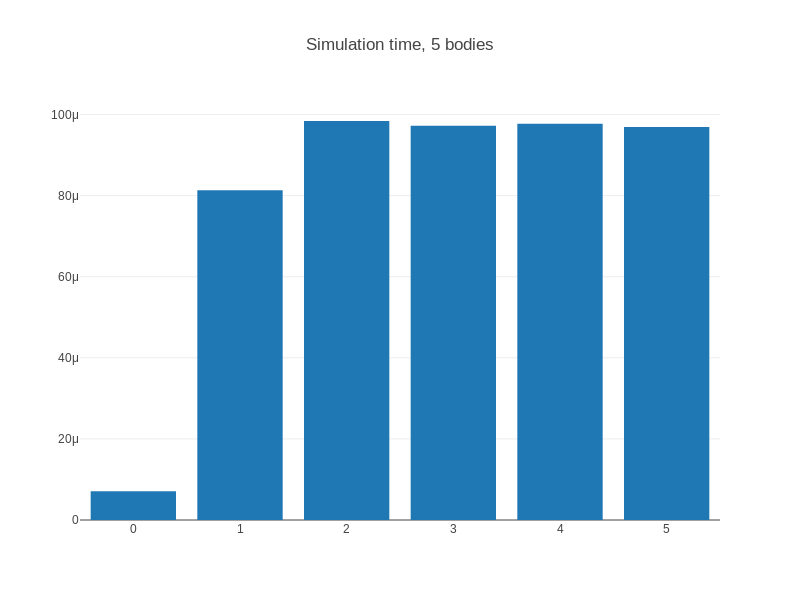
\includegraphics[width=\linewidth]{./grafiekskes/hist_simulation5.png}
    \caption{Simulatietijd 5 lichamen}
\end{figure}
\subsection{50 lichamen}
Vanaf 50 lichamen is de CPU nog steeds 2 - 3 keer sneller dan de GPU. Het aantal
lichamen stijgt waardoor de overhead ten opzichte van de hoeveelheid data
is verminderd. De verschillen tussen de OpenCL varianten zijn niet erg groot op
dit moment. Maar dit zal veranderen als het aantal lichamen nog stijgt.

\begin{figure}[H]
    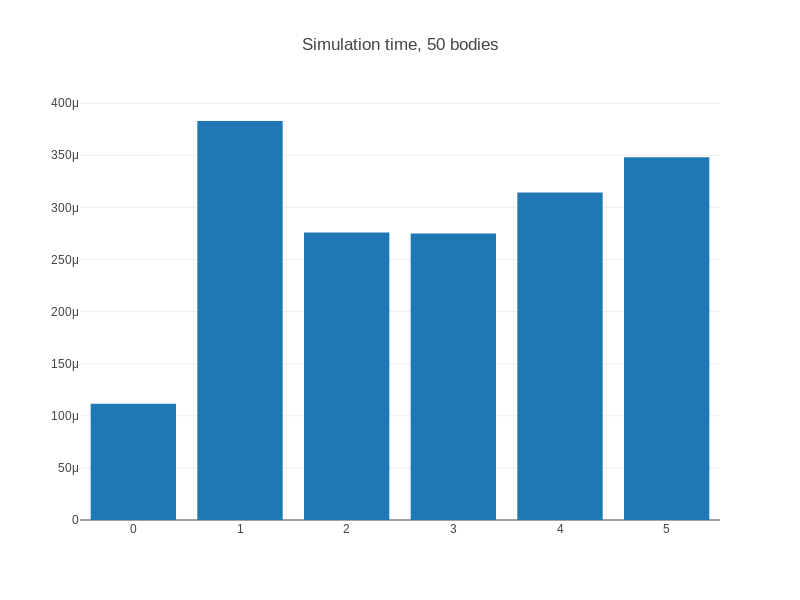
\includegraphics[width=\linewidth]{./grafiekskes/hist_simulation50.png}
    \caption{Simulatietijd 50 lichamen}
\end{figure}

\subsection{500 lichamen}
\label{hfd:lichamen-500}
Vanaf 500 lichamen bereiken we het breekpunt van de CPU, vanaf nu is de GPU sneller
om de gravitatie te simuleren dan de CPU.

\begin{itemize}
    \item Kernel 1 en 2 zijn niet-atomisch uitgevoerd (zie \ref{hfd:niet-atomisch-for1} en \ref{hfd:niet-atomisch-for2}) waardoor kernel 2 zijn performantie hoger is dan zijn atomische variant.
    Maar kernel 2 heeft last van \textit{race condities} wat dus foutieve resultaten oplevert.
    \item Kernel 3 lost de \textit{race condities} op van kernel 2, hierdoor is deze wel trager maar levert hij wel de juiste resultaten op.
    \item Kernel 4 is gelijkaardig aan kernel 1, de oorzaak hiervan is dat we de atomische operaties ook getest hebben op for-lus \ref{code:for2} (zie \ref{hfd:atomisch-for2}).
    Maar aangezien deze geen \textit{race condities} bevat, zien we ook geen verschil in performantie. Enkel de kleine for-lus \ref{code:for2} op de GPU draaien heeft dus weinig zin.
    \item Kernel 5 presteert duidelijk beter als zijn voorgangers. Door de combinatie te maken van beide for-lussen (zie \ref{hfd:combinatie-lussen}) verkrijgen we een betere performantie
    omdat alles op de GPU berekent werd. Deze kernel combineert eigenlijk kernel 3 en 4 waardoor het aantal dataoverdrachten stijgt.
    Deze zouden we nog kunnen optimaliseren, hierover later meer in paragraaf \ref{hfd:dataoverdrachten}.
\end{itemize}

\begin{figure}[H]
    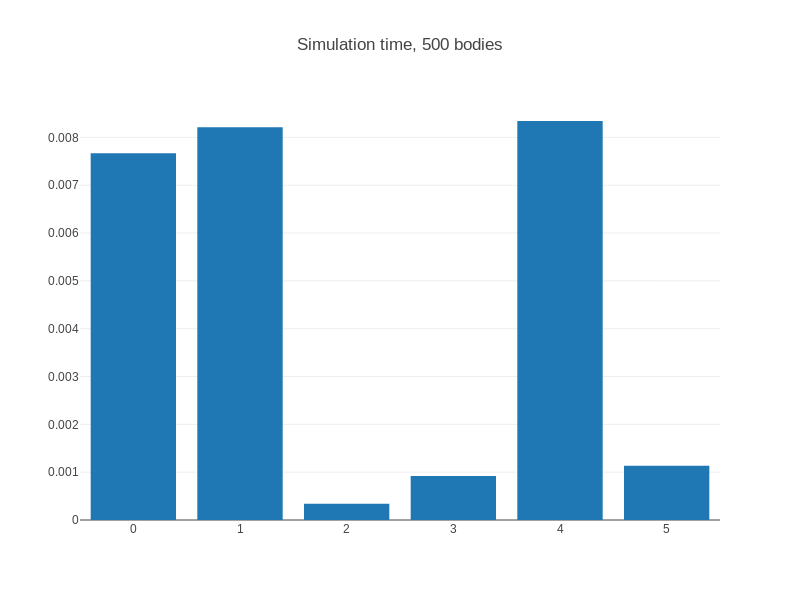
\includegraphics[width=\linewidth]{./grafiekskes/hist_simulation500.png}
    \caption{Simulatietijd 500 lichamen}
\end{figure}

\subsection{5~000 lichamen}
\begin{figure}[H]
    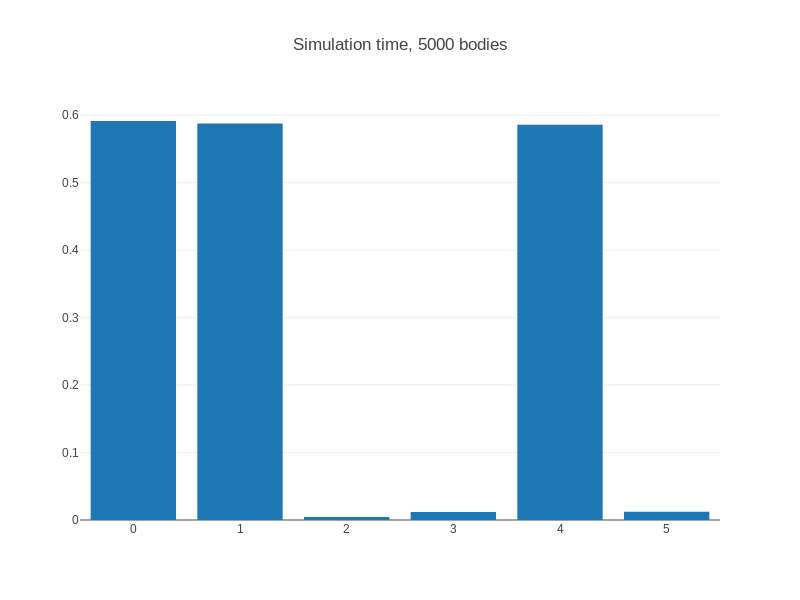
\includegraphics[width=\linewidth]{./grafiekskes/hist_simulation5000.png}
    \caption{Simulatietijd 5~000 lichamen}
\end{figure}

Hier zien we dezelfde trend als we reeds besproken hebben bij 500 lichamen (paragraaf \ref{hfd:lichamen-500}).
De kernels 2, 3 en 5 zijn beduidend sneller dan de CPU versie en kernels 1 en 4. Kernel 2 mogen we niet rekenen als
sneller omdat deze foutieve resultaten oplevert. Kernel 1 en 4 parallelliseren de kleine for-lus \ref{code:for2}
wat niet eg veel verbetering met zich meebrengt op vlak van performantie omdat de bewerking te kort is.

\begin{figure}[H]
    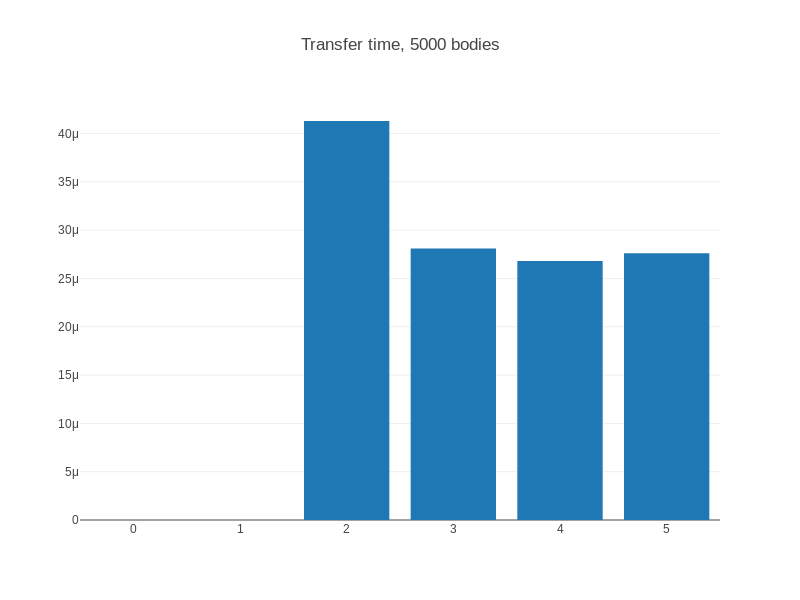
\includegraphics[width=\linewidth]{./grafiekskes/hist_transfer5000.png}
    \caption{Transfertijd 5~000 lichamen}
\end{figure}

% Nogal vreemd niet?? SIMON

% Zeveren over overdrachttijd van andere kernels?? SIMON
We zien duidelijk dat de transfertijd van kernel 4 veel meer is dan kernel 1.
\\
\\
\textit{Opmerking}: Er is geen transfertijd gemeten bij de CPU versie omdat er geen overdracht plaats vindt.

\subsection{50~000 lichamen}
\begin{figure}[H]
    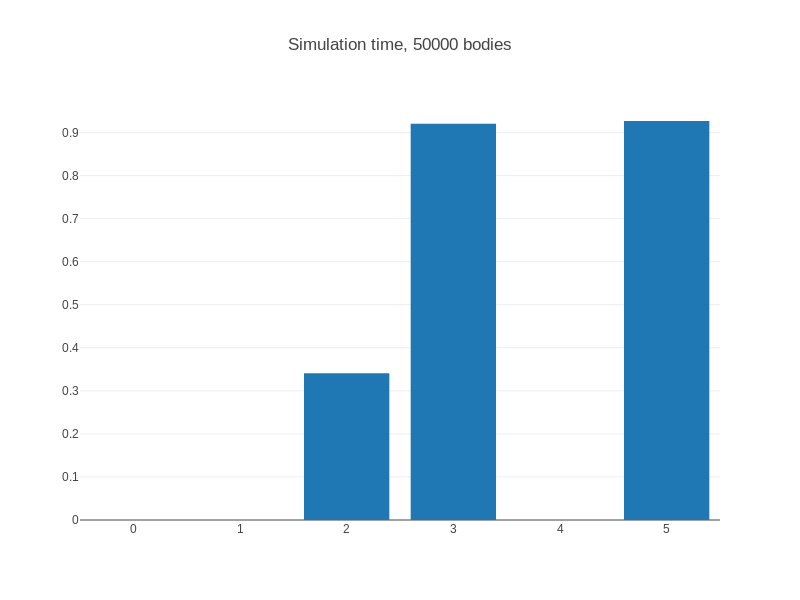
\includegraphics[width=\linewidth]{./grafiekskes/hist_simulation50000.png}
    \caption{Simulatietijd 50~000 lichamen}
\end{figure}

Vanaf 50~000 lichamen kunnen de CPU versie 0 en kernels 1 en 4 niet meer opstarten.
Kernels 3 en 5 leveren daarentegen nog steeds een uitstekende performantie, op
slechts 0.9 seconden kunnen zij de 50~000 lichamen berekenen. Dit is wel 100 maal
trager dan bij 5~000 lichamen, de oorzaak hiervan is de GPU hardware zelf. Deze was
op dat moment 100\% in gebruik. Het gevolg hiervan is dat de berekeningen in wachtrij
worden gezet tot de GPU klaar is voor de volgende taak.

Deze kernels leveren echter wel een groot verschil op in simulatietijd ten opzichte van de CPU versie
die bij 5~000 lichamen er al reeds 0.6 s over deed. Zij doen er slechts 0.9 s erover om
50~000 lichamen uit te rekenen. Het aantal lichamen vertienvoudigt maar de
simulatietijd stijgt slechts met 50\% ten opzichte van de CPU versie van 5~000 lichamen.

Bij 500 000 lichamen geven deze kernels het helaas ook op en vereisen deze ook nog
ingrijpende aanpassingen om de performantie te verhogen zoals we zullen bespreken in \ref{hfd:verbeteringen}.

\begin{figure}[H]
    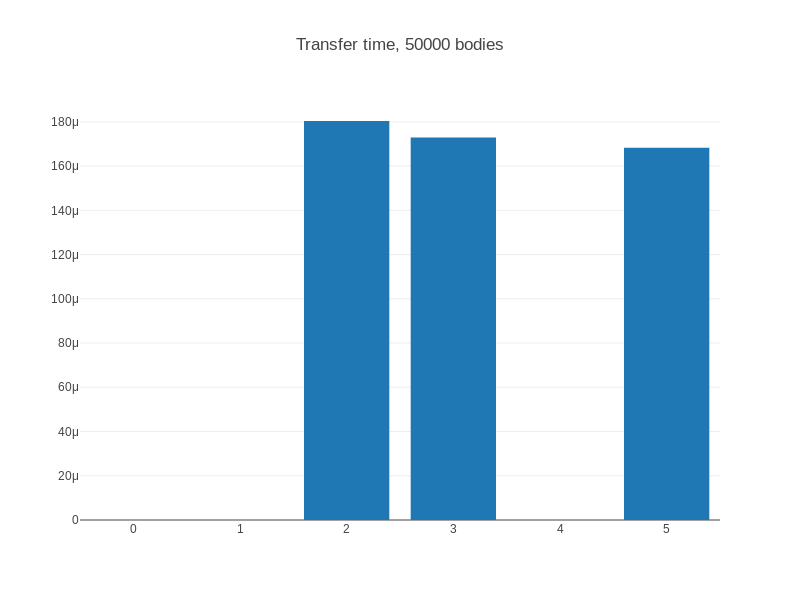
\includegraphics[width=\linewidth]{./grafiekskes/hist_transfer50000.png}
    \caption{Transfertijd 50~000 lichamen}
\end{figure}

Hier is heel duidelijk ook hoeveel impact de transfersnelheid heeft op het programma.
Tussen 5000 en 50000 bodies is de transfertijd soms 5 keer groter doordat er mee data
van en naar GPU gekopieerd moet worden.

%----------------------------------------------------------------------------------------
%	SECTION 4: IMPROVEMENTS
%----------------------------------------------------------------------------------------
\section{Mogelijke verbeteringen}
\label{hfd:verbeteringen}
Het is nog mogelijk om de laatste versie van het programma nog te versnellen door
gebruik te maken van nog enkele OpenCL functies en ontwerppatronen. Deze werden
niet ge\"{i}mplementeerd wegens tijdsgebrek.

\subsection{Minder dataoverdrachten}
\label{hfd:dataoverdrachten}
Het programma kopieert nu telkens per OpenCL kernel de data van de host naar de GPU en
omgekeerd. Dit resulteert in 4 dataoverdrachten, wat erg veel nutteloze
overhead is, omdat beide for-lussen draaien als een aparte kernel.

We zouden de for-lussen kunnen overzetten in \'{e}\'{e}n kernel waardoor de dataoverdrachten
worden gereduceerd tot slechts 2 overdrachten.

\subsection{Effici\"{e}nt opsplitsen in werkgroepen}
\label{hfd:werkgroepen}
Beide for-lussen worden simpel weg op de GPU uitgevoerd zonder dat het algoritme
geoptimaliseerd werd voor parrallelisme op de GPU. Dit resulteert in een slechter
gebruik van het geheugen (globaal i.p.v. lokaal) waardoor de berekeningen trager
kunnen verlopen door het geheugen bottleneck.

Elke processor kan aan de hele dataset. Beter gezegd: het geheugen is volledig
gedeeld onder elke processor. Hierdoor staat dit globaal geheugen verder weg
van de processor kern en duurt het dus langer vooraleer de data arriveert bij
de processor.

Als we gebruik maken van het lokaal geheugen van een werkgroep kunnen we dit probleem
voorkomen. Maar dit vereist tevens ook dat we de berekeningen zodanig kunnen opsplitsen
zodat ze in een werkgroep passen.

\subsection{Coalesced memory access}
Indien we het programma zouden optimaliseren om zijn geheugentoegangen te limiteren
tot zijn buren kunnen we een hogere snelheid halen omdat de naburige werkitems
sneller toegankelijk zijn dan werkitems die aan de andere kant van de GPU liggen.
Maar dit vereist opnieuw een ingreep op het algoritme zoals reeds besproken in
\ref{hfd:werkgroepen}, welke iets uitgebreider is omdat men rekening moet houden
met de buren van elk workitem.

%----------------------------------------------------------------------------------------
%	SECTION 5: CONCLUSION
%----------------------------------------------------------------------------------------
\section{Conclusie}

We hebben het n-body probleem stapsgewijs geprobeert te parallelliseren met behulp
van OpenCL, dit is vrij aardig gelukt aangezien we met onze kernel 10 keer zoveel lichamen
kan berekenen ten opzichte van de CPU versie zonder al veel te moeten inboeten op vlak
van performantie.
%----------------------------------------------------------------------------------------
\end{document}
